\section{Storage systems}

The storage systems can be classified as: 
\begin{itemize}
    \item \textit{Direct Attached Storage} (DAS): these storage systems are directly linked to a server or workstation, appearing as disks/volumes within the client operating system.
    \item \textit{Network Attached Storage} (NAS): NAS entails a computer connected to a network, offering file-based data storage services (e.g., FTP, network file system, and SAMBA) to other devices on the network. 
        It is recognized as a File Server by the client operating system.
    \item \textit{Storage Area Networks} (SAN): SAN comprises remote storage units connected to servers through specific networking technologies (e.g., fiber channel). 
        They are perceived as disks/volumes by the client operating system.
\end{itemize}
\begin{figure}[H]
    \centering
    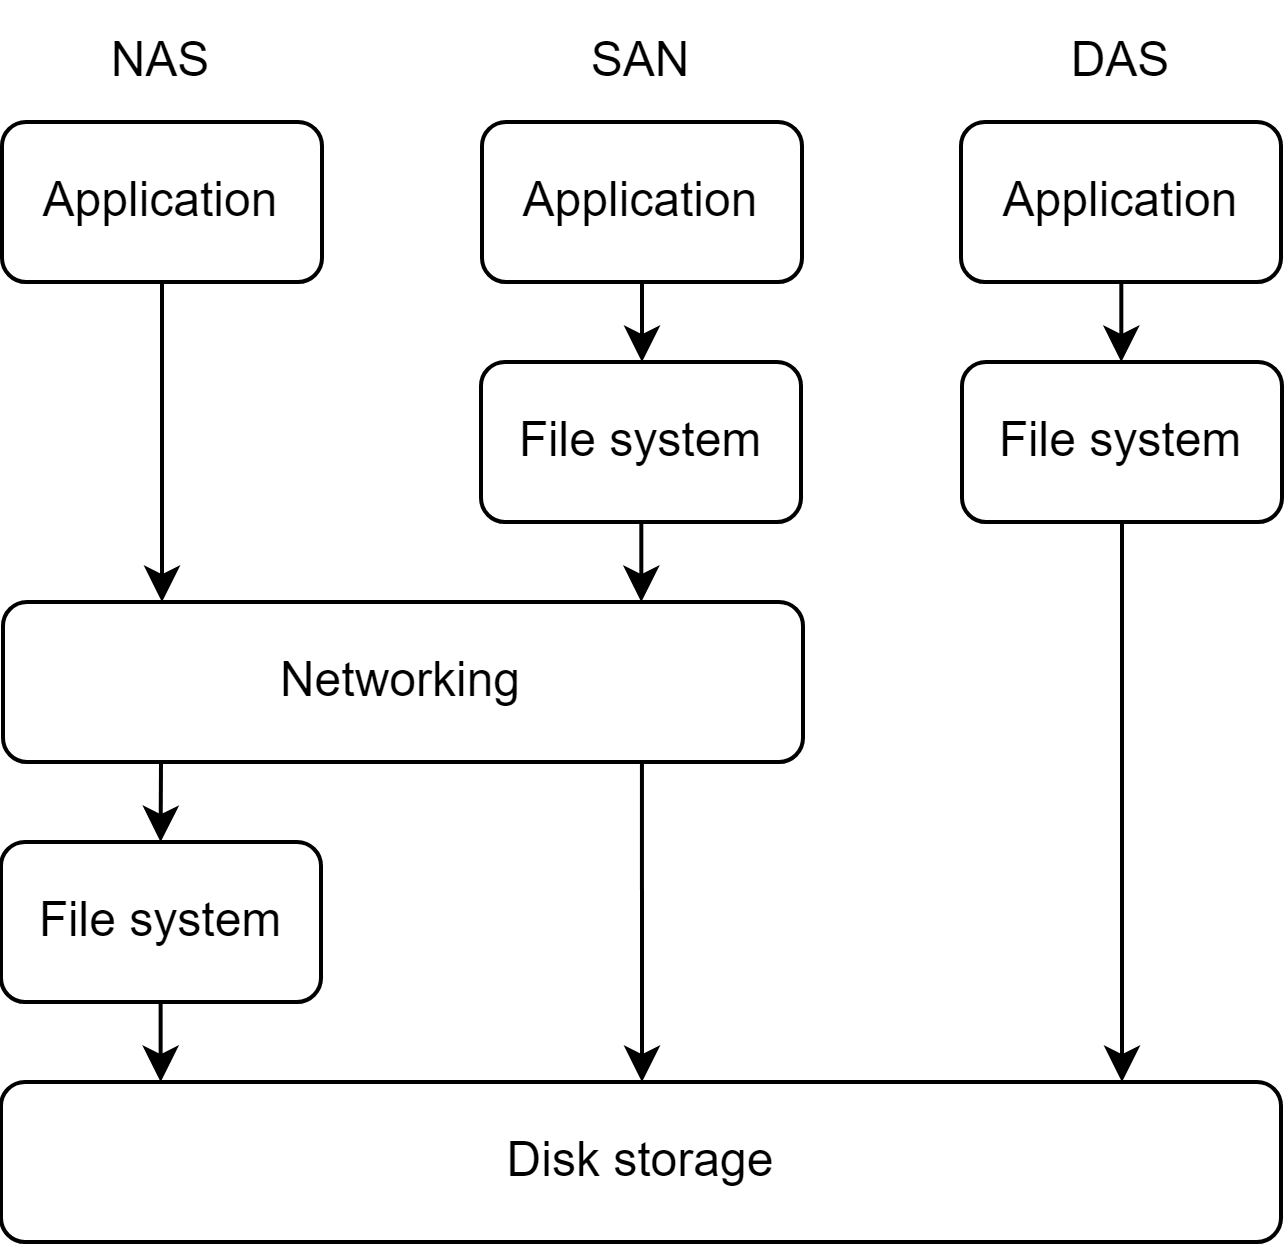
\includegraphics[width=0.4\linewidth]{images/ssc.png}
    \caption{Storage system classification}
\end{figure}

\subsection{Direct Attached Storage}
Direct Attached Storage (DAS) refers to a storage system directly connected to a server or workstation. 
It serves to distinguish non-networked storage from Storage Area Networks (SAN) and Network Attached Storage (NAS). 
Key characteristics of DAS include limited scalability and complex manageability. 
Accessing files from other machines typically requires utilizing the file sharing protocol of the operating system.

DAS can be internal or external; it does not exclusively entail internal drives. 
Any external disks connected via a point-to-point protocol to a PC can be classified as DAS.
\begin{figure}[H]
    \centering
    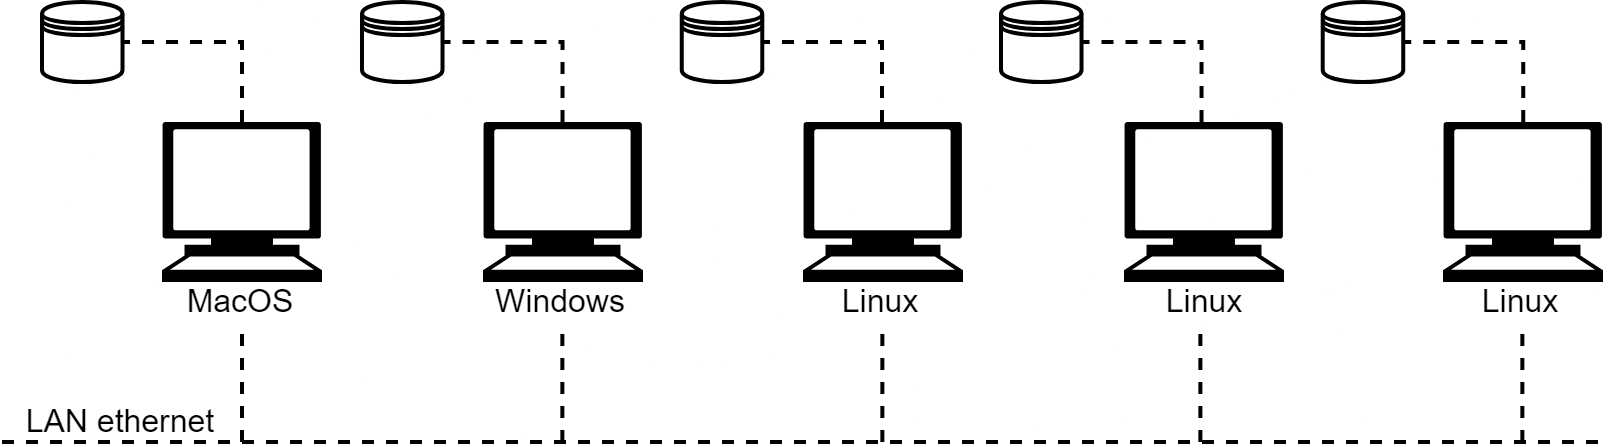
\includegraphics[width=0.4\linewidth]{images/das.png}
    \caption{Direct Attached Storage architecture}
\end{figure}


\subsection{Network Attached Storage}
A Network Attached Storage (NAS) unit is a computer connected to a network, offering file-based data storage services exclusively to other devices within the network. 
NAS systems typically comprise one or more hard disks, often configured into logical redundant storage containers or RAID setups. 
They provide file-access services to hosts connected via TCP/IP networks through protocols like Networked File Systems or SAMBA. 
Each NAS element is assigned its own IP address, facilitating individual identification and management.

NAS systems exhibit good scalability, allowing for the addition of devices within each NAS element or the expansion of the number of NAS elements themselves.
\begin{figure}[H]
    \centering
    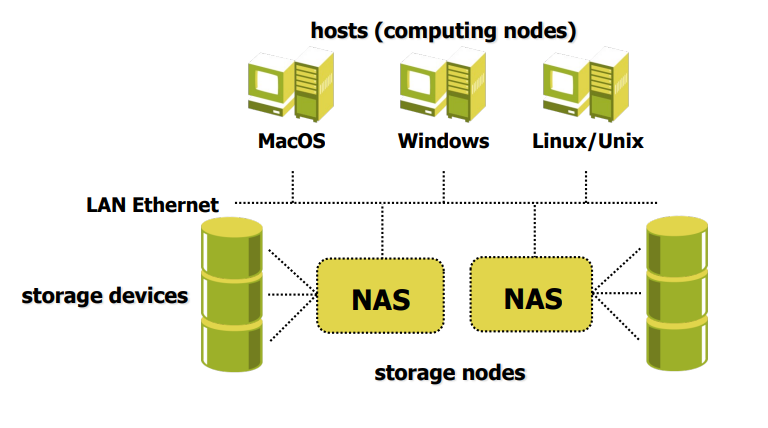
\includegraphics[width=0.4\linewidth]{images/nas.png}
    \caption{Network Attached Storage architecture}
\end{figure}

\paragraph*{NAS and DAS}
The primary distinctions between Network Attached Storage (NAS) and Direct Attached Storage (DAS) are as follows:
\begin{itemize}
    \item DAS serves as a mere extension of an existing server and may not necessarily be networked.
    \item NAS is purposefully designed as a convenient and self-contained solution for sharing files across a network.
    \item The performance of NAS primarily relies on the speed and congestion levels of the network.
\end{itemize}

\subsection{Storage Area Network}
Storage Area Networks (SANs) are remote storage units connected to PCs/servers through specific networking technologies. 
SANs feature a dedicated network solely devoted to accessing storage devices, typically comprising two distinct networks: one for TCP/IP communication and another dedicated network, like fiber channel. 
They offer high scalability by simply increasing the number of storage devices connected to the SAN network.
\begin{figure}[H]
    \centering
    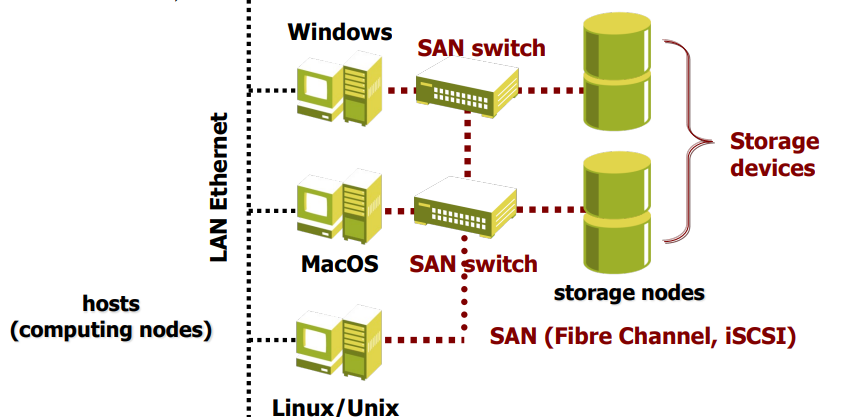
\includegraphics[width=0.4\linewidth]{images/san.png}
    \caption{Storage Area Network architecture}
\end{figure}

\paragraph*{NAS and SAN}
AS provides both storage and a file system, contrasting with SAN, which solely offers block-based storage, leaving file system concerns on the client side. 
A way to loosely differentiate NAS from SAN is:
\begin{itemize}
    \item NAS presents itself to the client OS as a file server, allowing the client to map network drives to shares on that server.
    \item A disk accessible through SAN appears to the client OS as a disk, visible in disk and volume management utilities alongside the client's local disks, and available for formatting with a file system.
\end{itemize}
Traditionally:
\begin{itemize}
    \item NAS is utilized for low-volume access to a large amount of storage by many users.
    \item SAN serves as the solution for petabytes ($10^{12}$) of storage and simultaneous access to files, such as streaming audio/video.
\end{itemize}

\subsection{Summary}
\begin{figure}[H]
    \centering
    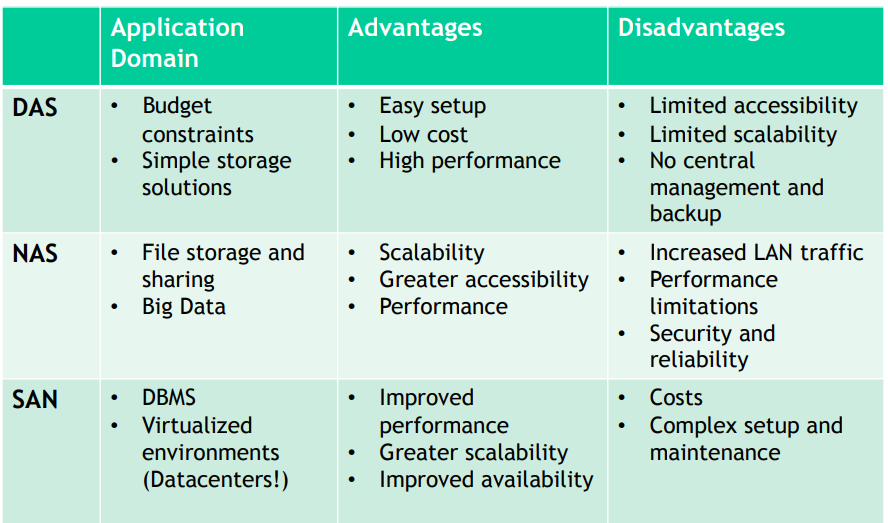
\includegraphics[width=1\linewidth]{images/stor.png}
\end{figure}